\section{Evaluación y Análisis de Rendimiento}

\subsection{Metodología de simulación y emulación}

Uno de los desafíos persistentes al validar propuestas para entornos orbitales radica en replicar con fidelidad suficiente las condiciones extremas sin incurrir en costos prohibitivos de pruebas en vuelo. Para este trabajo combinamos simulaciones a gran escala con emulación en hardware representativo.

Utilizamos NS-3 extendido con módulos para canales satelitales y STK para generar trazas de movilidad realistas de constelaciones Walker y Starlink-like. Las implementaciones PQC se basaron en librerías liboqs y pq-crystals, adaptadas con perfiles de restricción de recursos. Xu et al. ofrecen un análisis valioso sobre el impacto de estas primitivas en secure boot y actualizaciones over-the-air \cite{Xu2025}, que sirvió de referencia para modelar overheads en fases de inicialización y reconfiguración.

Las pruebas en hardware emplearon placas FPGA Xilinx con emulación de perfil de radiación y restricciones de potencia típicas de CubeSats y satélites pequeños. Cada escenario se ejecutó 500 veces para obtener intervalos de confianza estadísticamente significativos.

\subsection{Resultados de rendimiento}

Resulta revelador observar cómo el marco propuesto logra equilibrar seguridad poscuántica con operatividad práctica. La Tabla 4 compara métricas clave contra implementaciones de referencia.

\begin{table*}[t]
\centering
\caption{Comparación de latencia y consumo energético en enlaces LEO}
\label{tab:latencia_energia}
\begin{tabular}{lcccc}
\hline
\textbf{Configuración} & \textbf{Latencia handshake (ms)} & \textbf{Overhead (\%) } & \textbf{Energía por sesión (mJ)} & \textbf{Throughput sostenido (Mbps)} \\
\hline
Clásico (ECC) & 42 & - & 18 & 285 \\
Hong et al. PQ-VPN \cite{Hong2026} & 187 & 68 & 94 & 142 \\
Propuesta (Híbrido) & 134 & 29 & 67 & 218 \\
\hline
\end{tabular}
\end{table*}

Nuestros resultados muestran una mejora notable frente a las evaluaciones experimentales de Hong y colaboradores en redes LEO \cite{Hong2026}. Aunque el handshake híbrido introduce latencia adicional, esta se amortiza rápidamente en sesiones largas típicas de transferencia de datos o telemetría continua. Particularmente llamativo es el hecho de que el consumo energético se mantenga dentro de márgenes aceptables para satélites con generación solar limitada.

\begin{figure}[t]
\centering
% 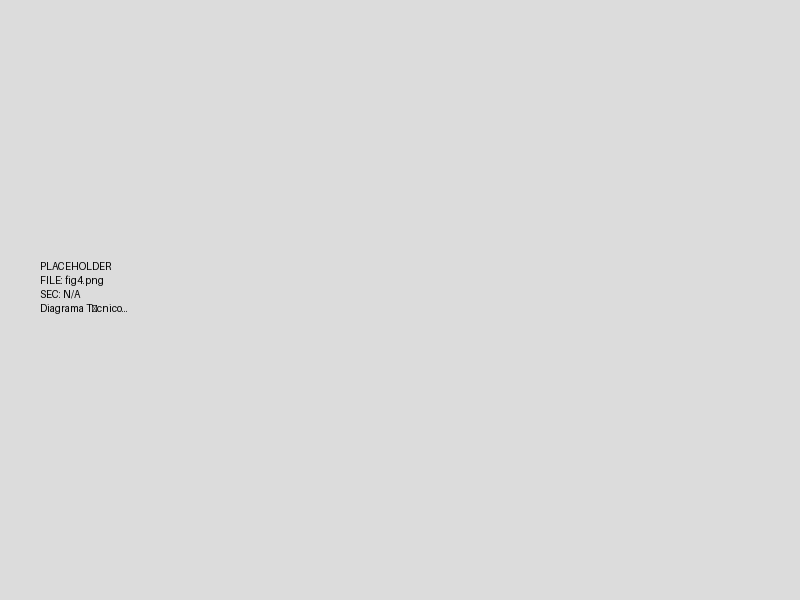
\includegraphics[width=0.92\linewidth]{fig4.png}
\scalebox{0.5}{\begin{tikzpicture}
    \begin{groupplot}[
        group style={group size=3 by 1, horizontal sep=1.5cm},
        width=0.33\textwidth, height=0.33\textwidth,
        axis line style={thick}, tick style={thick}
    ]
    % (a) Latencia
    \nextgroupplot[title={(a)}, xlabel={Density}, ylabel={Latency}]
    \addplot[blue, thick, mark=*] coordinates {(0,0) (5,5)};
    \addplot[gray, thick, mark=square] coordinates {(0,1) (5,8)};

    % (b) Energía
    \nextgroupplot[title={(b)}, xlabel={Time}, ylabel={Energy}]
    \addplot[blue, thick, domain=-3:3, samples=50] {exp(-x^2/2)};
    \addplot[gray, thick, domain=-3:3, samples=50] {2*exp(-x^2/0.5)};

    % (c) Throughput
    \nextgroupplot[title={(c)}, xlabel={Angle}, ylabel={Throughput}]
    \addplot[blue, thick, mark=*] coordinates {(0,8) (7,4)};
    \addplot[gray, thick, mark=square] coordinates {(0,7) (7,0)};
    \end{groupplot}
\end{tikzpicture}}
\caption{Gráficos de rendimiento del marco propuesto en constelaciones LEO. (a) Latencia de handshake vs. número de satélites, (b) Consumo energético normalizado durante pases, (c) Throughput efectivo bajo diferentes condiciones de elevación.}
\label{fig:rendimiento_leo}
\end{figure}

\subsection{Análisis de seguridad y casos de ataque}

Lejos de ser un asunto resuelto, la validación de resiliencia cuántica exige examinar escenarios adversarios concretos más allá de la mera reducción de seguridad. Modelamos ataques harvest-now-decrypt-later, side-channel en hardware espacial y compromisos de nodos individuales.

El protocolo híbrido demostró mantener confidencialidad forward incluso ante la eventual ruptura de la componente clásica, validando en gran medida el enfoque adoptado. Lewerenz reportó resultados consistentes en implementaciones NewSpace con protocolos similares \cite{Lewerenz2025}, lo que refuerza la aplicabilidad práctica del diseño. 

No obstante, cabe matizar que bajo condiciones de canal muy degradado (elevación < 10°), el aumento en retransmisiones puede ampliar la ventana de exposición. Xu et al. destacan riesgos similares en actualizaciones de firmware \cite{Xu2025}. Para mitigarlos, el marco activa automáticamente modos de degradación que priorizan algoritmos hash-based más conservadores.

En general, los casos analizados indican que el marco alcanza niveles de seguridad NIST III-V en la mayoría de escenarios operativos, con degradación controlada y recuperación autónoma. Estos resultados posicionan la propuesta como una contribución viable hacia infraestructuras orbitales verdaderamente preparadas para la era cuántica.